\documentclass[11pt,a4paper]{article}

\usepackage[utf8]{inputenc}
\usepackage[T1]{fontenc}
\usepackage[english]{babel}
\usepackage[a4paper,margin=2.4cm]{geometry}

\usepackage{amsmath, amssymb, amsthm}
\usepackage{mathtools}
\usepackage{stmaryrd}
\usepackage{booktabs}
\usepackage{tabularx}
\usepackage{array}
\usepackage{caption}
\usepackage{subcaption}
\usepackage{float}
\usepackage{enumitem}
\usepackage{microtype}
\usepackage{xcolor}
\usepackage{listings}
\usepackage{fancyhdr}
\usepackage{titlesec}
\usepackage{graphicx}
\usepackage{tikz}
\usetikzlibrary{positioning, arrows.meta, fit, backgrounds, calc, shapes.geometric}
\usepackage[hidelinks]{hyperref}

%  ---  Palette shared with the companion reports  ---
\definecolor{ink}{RGB}{26,30,36}
\definecolor{slate}{RGB}{92,101,112}
\definecolor{mist}{RGB}{233,235,238}
\definecolor{rulegrey}{RGB}{188,194,201}
\definecolor{steel}{RGB}{47,72,102}
\definecolor{steellight}{RGB}{124,146,172}
\definecolor{signal}{RGB}{160,32,45}
\definecolor{southc}{RGB}{51,115,204}
\definecolor{northc}{RGB}{230,128,38}
\definecolor{knows}{RGB}{26,140,70}

\hypersetup{
    colorlinks=true,
    linkcolor=steel,
    citecolor=steel,
    urlcolor=steel,
    pdftitle={Maps That Go Stale},
    pdfauthor={Haniel Ulises},
}

\color{ink}

\setlength{\headheight}{22pt}
\pagestyle{fancy}
\fancyhf{}
\fancyhead[L]{\small\textcolor{slate}{\itshape Maps That Go Stale}}
\fancyhead[R]{\small\textcolor{slate}{\thepage}}
\renewcommand{\headrulewidth}{0.4pt}
\renewcommand{\headrule}{\hbox to\headwidth{\color{rulegrey}\leaders\hrule height \headrulewidth\hfill}}

\titleformat{\section}{\normalfont\large\bfseries\color{ink}}{\thesection}{0.7em}{}
\titleformat{\subsection}{\normalfont\normalsize\bfseries\color{ink}}{\thesubsection}{0.7em}{}
\titleformat{\paragraph}[runin]{\normalfont\bfseries\color{slate}}{}{0em}{}[.]

\captionsetup{font=small, labelfont={bf,color=slate}, textfont=footnotesize}

\theoremstyle{definition}
\newtheorem{definition}{Definition}
\newtheorem{proposition}{Proposition}
\newtheorem{lemma}{Lemma}
\newtheorem{corollary}{Corollary}
\newtheorem{fact}{Fact}
\newtheorem{remark}{Remark}

\lstdefinestyle{sys}{
    backgroundcolor=\color{mist},
    basicstyle=\ttfamily\scriptsize\color{ink},
    keywordstyle=\color{steel}\bfseries,
    commentstyle=\color{slate}\itshape,
    stringstyle=\color{slate},
    morecomment=[l]{;},
    morekeywords={:types,:predicates,:objects,:agents,:goal,:init,:event,:action,:action-type,:observability-conditions,:precondition,:effects,:events,:relations,:designated,:conditions,:observability-types},
    frame=single,
    rulecolor=\color{rulegrey},
    framesep=5pt,
    xleftmargin=6pt,
    xrightmargin=0pt,
    breaklines=true,
    showstringspaces=false,
    columns=fullflexible,
    captionpos=b,
}
\lstset{style=sys}

%  ---  Notation  ---
\newcommand{\Ag}{\mathcal{A}}
\newcommand{\Mod}{\mathcal{M}}
\newcommand{\Ev}{\mathcal{E}}
\newcommand{\prd}{\otimes}
\newcommand{\Kop}[1]{K_{#1}}
\newcommand{\Eop}[1]{E_{#1}}
\newcommand{\Cop}[1]{C_{#1}}
\newcommand{\Kw}[1]{\mathit{Kw}_{#1}}
\newcommand{\code}[1]{\texttt{\small #1}}
\newcommand{\ag}[1]{\mathit{#1}}
\newcommand{\job}{\mathit{job}}
\newcommand{\pre}{\mathit{pre}}
\newcommand{\post}{\mathit{post}}
\newcommand{\dist}{\mathrm{dist}}
\newcommand{\depth}{\mathrm{depth}}
\newcommand{\atview}{\mathit{at\text{-}view}}
\newcommand{\sem}[1]{\llbracket #1 \rrbracket}

\newcommand{\blocked}{\mathit{blocked}}
\newcommand{\sees}{\mathit{sees}}
\newcommand{\Bop}[1]{B_{#1}}
\newcommand{\Obs}{O}
\newcommand{\shift}{\sigma}
\begin{document}

\begin{titlepage}
\centering
\vspace*{2.4cm}
{\color{rulegrey}\rule{\textwidth}{0.8pt}}\\[0.9cm]
{\LARGE\bfseries Maps That Go Stale\par}
\vspace{0.5cm}
{\large\color{slate} Stale Maps as False Beliefs, and a Received Map as an Update,\\
for a Fleet of Eight Robots\par}
\vspace{0.7cm}
{\color{rulegrey}\rule{\textwidth}{0.8pt}}\\[1.4cm]

{\large Haniel Ulises\par}
\vspace{0.3cm}
{\color{slate} Epistemic Robotics}\\
\vspace{0.15cm}
{\color{slate}\today}

\vfill
{\color{slate}\small
Eight robots begin a shift holding the same occupancy map of a warehouse floor.
A forklift stages a load in one bay and clears another, and a robot sees a
change only when its station has a sight line into the bay. Every other robot
maps the change onto nothing having changed, the static-world assumption every
occupancy map is built on, and its map goes stale without its knowing. We state
this as an epistemic planning task in which a stale map is a false belief and a
map sent from one robot to another is an action of its own.

\vspace{0.6em}
We prove that after the forklift the model gives every robot exactly the map its
station leaves it, with four worlds whatever the size of the fleet; that a
received map taken as a fact leaves a robot whose map says otherwise believing
every formula; that the same map taken as news that the bay changed is an update
in the sense of Katsuno and Mendelzon, which changes the recipient's belief about
one bay and nothing else; that a robot with a stale reading believes every other
robot shares it, so a precondition requiring the sender to believe the receiver
holds the opposite never lets a stale reading be sent; and that bringing every
map up to date takes at least one message per stale entry. Aletheia's policies
meet these bounds: three messages to the three haulers that need one, or eleven,
one per stale entry. Random fleets solve to 32 robots and not, within 600\,s, at
64. In Gazebo, four fleets of eight robots ran on the same floor. The fusion this
repository has, which settles a contradiction by confidence, repaired nothing,
since 0 against 100 is a tie; sharing every map with the sender's reading or with
observation times delivered with 168 messages; the plan delivered with 3, and the
epistemic state's beliefs agreed with the robots' maps on all 24.}
\vspace{1.2cm}
\end{titlepage}

\tableofcontents
\newpage

%  ======================================================================
\section{Scope}
\label{sec:scope}

The pass-through report~\cite{ulises2026pt} reads what a robot knows off the map
it builds and treats an exchange of maps as an announcement. Its maps only ever
gain information: nothing on its floor changes after a robot has looked. This
report takes the case in which the floor changes after it was mapped, and a map
becomes wrong. That is a problem every map shared across a fleet has, and it is
the case in which an occupancy grid's own update rule and the logic of belief
disagree about what a received map should do. The false-belief
report~\cite{ulises2026fb} treats one robot that misses one change; here eight
robots miss different changes, and no robot holds a current map.

Five claims are advanced.

\begin{enumerate}[leftmargin=1.4em, itemsep=2pt]
  \item After the forklift every robot believes exactly the map its station
        leaves it, and the model has four worlds for any fleet
        (Proposition~\ref{prop:model}).
  \item A received map taken as a fact leaves a robot whose map says otherwise
        with no world (Proposition~\ref{prop:collapse}); taken as news that the
        bay changed it is an update, which changes the recipient's belief about
        one bay and no robot's belief about any other (Proposition~\ref{prop:update}).
  \item A robot with a stale reading of a bay can send it to no robot under the
        precondition $\Bop{i}\Bop{j}$ of the opposite (Proposition~\ref{prop:guard}).
  \item Bringing every map up to date takes at least one message per stale entry,
        and the planner's policy sends exactly that many
        (Proposition~\ref{prop:least}).
  \item On the floor, four fleets differing only in how they share maps did what
        an analysis made before they ran said they would; the fusion the
        repository has repairs no stale map (Lemma~\ref{lem:tie}).
\end{enumerate}

Three bounds are stated at the outset. The robots localise by odometry, which in
simulation is the world frame, so the mapping is mapping with known poses over a
prior; a robot that did not know where it is would not know which bay it saw.
Who sees each change is a geometric claim about the floor plan, checked by
casting rays and confirmed on every run by the robots' own maps, not assumed of
the lasers. And every map sent arrives: a lossy link is the subject of the
link-outage report.

%  ======================================================================
\section{Preliminaries}
\label{sec:prelim}

The definitions are those of the companion reports: epistemic models
$\Mod = (W, R, V, W_d)$ with one relation $R_a$ per agent, event models with
observability types, and their product update $\Mod \prd \Ev$, in which
$(w,e)$ is a world when $\Mod, w \models \pre(e)$, its valuation is $e$'s
postconditions applied to $w$'s, and $(w,e) \mathrel{R'_a} (v,f)$ iff
$w \mathrel{R_a} v$ and $(e,f) \in Q_a$, where $Q_a$ is the relation of the
observability type agent $a$ has for the action. $\Bop{a}\varphi$ holds at $w$
when $\varphi$ holds at every $v$ with $w \mathrel{R_a} v$; on a $\mathrm{KD45}$
frame it is belief, and an agent with no successor at $w$ believes every formula.

Two observability types are used throughout. \emph{Fully} relates every event to
itself. \emph{Oblivious} relates every event to a designated null event, or to
the action's event in which nothing changes; an oblivious agent's worlds after
the update are copies of its worlds before it.

\begin{lemma}[Oblivious agents]
\label{lem:oblivious}
If every event's relation for agent $a$ is to an event $n$ with trivial
postconditions that occurs at every world, then the worlds reachable from
$(w,e)$ by $a$ are the pairs $(v,n)$ with $w \mathrel{R_a} v$, and the part of
$\Mod \prd \Ev$ reachable from them through agents that relate $n$ to $n$ is
isomorphic to the part of $\Mod$ reachable from those $v$.
\end{lemma}

\begin{proof}
$(w,e) \mathrel{R'_a} (v,f)$ iff $w \mathrel{R_a} v$ and $f = n$, and $(v,n)$
exists since $n$ occurs everywhere. If every agent relates $n$ only to $n$,
$(v,n) \mapsto v$ is a bijection onto the worlds reachable from $v$ that
preserves every relation and, $n$'s postconditions being trivial, every
valuation.
\end{proof}

%  ======================================================================
\section{The domain}
\label{sec:domain}

The agents are robots $r_1, \dots, r_N$; three of the eight on the floor haul.
The bays are $t_1, t_2, t_3$. The atoms are $\blocked(t)$; the static
$\sees(i,t)$, that robot $i$'s station has a sight line into bay $t$;
$\mathit{hauls}(i)$ and $\mathit{delivered}(i)$; the forklift's schedule,
$\mathit{stage\text{-}due}(t)$ and $\mathit{clear\text{-}due}(t)$; and two that
tell the floors apart, $\mathit{radio}$ and $\mathit{doubts}$. The initial model
is one world, every fact of it common knowledge: the shift map
$\shift$, in which $t_1$ is open and $t_2, t_3$ are blocked, the stations' sight
lines, the roles and the schedule. Whether the forklift will use its slots is the
one thing not known in advance, and the instance does not say it in the initial
state: the forklift's actions do.

\begin{table}[H]
\centering\small
\begin{tabularx}{\textwidth}{@{}l l X X@{}}
\toprule
action & type & events & observability \\
\midrule
$\mathit{stage}(t)$, $\mathit{clear}(t)$ & change & the change; the slot passing with nothing changed & Fully if $\sees(i,t)$, Oblivious to the slot otherwise \\
$\mathit{send\text{-}open}(i,j,t)$ & map report & the report; the change it implies; null & $i$ Fully, $j$ Recipient, the rest Oblivious \\
$\mathit{look}(i,t)$ & private sensing & open; blocked; null & $i$ Fully, the rest Oblivious \\
$\mathit{cross}(h,t)$ & private ontic & $\mathit{delivered}(h)$; null & $h$ Fully, the rest Oblivious \\
\bottomrule
\end{tabularx}
\caption{The actions. $\mathit{send\text{-}blocked}$ is $\mathit{send\text{-}open}$
with the reading reversed; $\mathit{look}$ applies only on the doubting floor,
where a robot that does not see a change relates the change and the slot, and is
uncertain instead of wrong.}
\label{tab:actions}
\end{table}

The preconditions carry the epistemic content:
\begin{align*}
\pre(\mathit{send\text{-}open}(i,j,t)) &= \mathit{radio} \wedge \Bop{i}\neg\blocked(t) \wedge \Bop{i}\Bop{j}\blocked(t),\\
\pre(\mathit{cross}(h,t)) &= \mathit{hauls}(h) \wedge \neg\blocked(t) \wedge \Bop{h}\neg\blocked(t).
\end{align*}
The map report has three events: $\mathit{told}$, with the precondition above and
trivial postconditions, designated; $\mathit{revise}$, with precondition
$\blocked(t)$ and postcondition $\neg\blocked(t)$; and the null event. The
recipient's type relates $\mathit{told}$ and $\mathit{revise}$ to
$\mathit{revise}$, and null to null. The report is the false-belief report's
action type~\cite{ulises2026fb}, generalised to a fleet with every other robot
oblivious.

Four floors are written for any fleet by \code{tools/stale\_maps.py}. On the
\emph{radio} floor the goal is that every hauler has delivered. On the
\emph{silent} floor there is no radio. On the \emph{doubt} floor there is no
radio, and robots know their maps may go stale. On the \emph{resync} floor the
goal is that every robot believes every bay as it is.

%  ======================================================================
\section{The floor}
\label{sec:floor}

\begin{figure}[H]
\centering
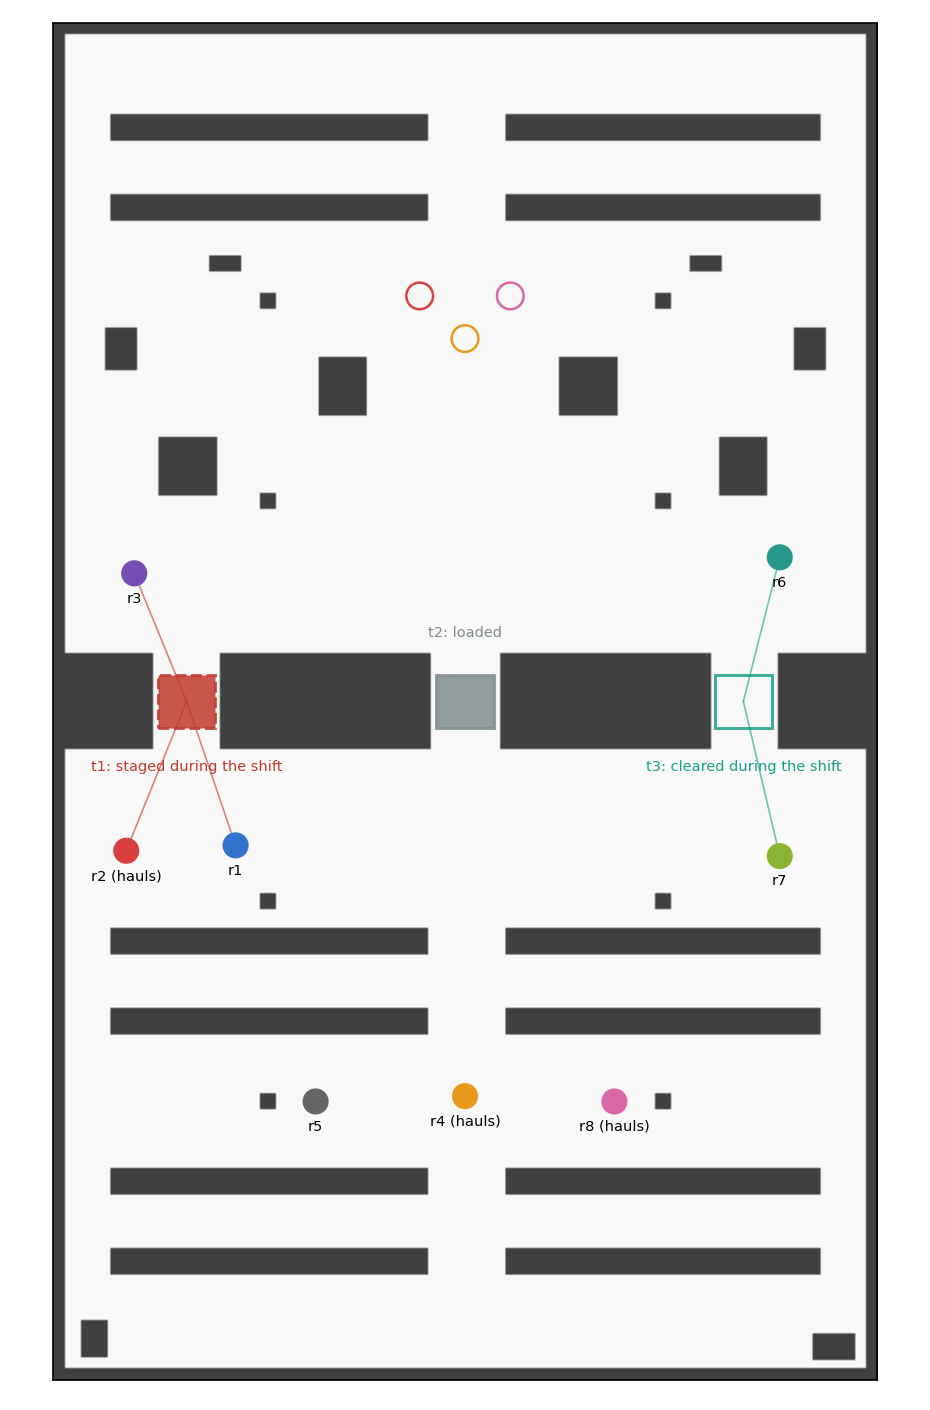
\includegraphics[width=0.42\textwidth]{figures/stale_maps_floor.png}
\caption{The pass-through floor with eight stations. $t_1$, dashed, is staged
during the shift; $t_3$ is cleared; $t_2$ keeps its load. A line joins a station
to each change it sees. $r_2$, $r_4$ and $r_8$ haul to the rings north of the
racking.}
\label{fig:floor}
\end{figure}

The hall and the racking block with its three bays are the pass-through
floor's~\cite{ulises2026pt}. \code{tools/check\_floor.py} tests three claims on
the floor plan before anything runs, by casting rays over its occupied cells with
the other robots standing at their stations as discs, or by flooding its free
cells inflated by the driver's 0.35\,m.

\begin{fact}[Sight]
\label{fact:sight}
A load staged in a bay is in view of a station with at least fifteen of its cells
or with none, and a cleared bay with every cell the load covered or with none,
within the laser's 12\,m. $t_1$'s change is seen from the stations of
$r_1, r_2, r_3$; $t_3$'s from those of $r_6, r_7$; no station sees both.
\end{fact}

The two thresholds follow the reading a map makes of a bay: blocked when any cell
of its corridor is occupied, clear when every cell is free. One cell of a staged
load decides it; a cleared bay is decided only when every cell the load covered
has been seen free, and a station that saw part of it would hold a reading
neither the shift map's nor the floor's.

\begin{fact}[Routes]
A hauler whose map is current reaches its drop through $t_3$ and through no other
bay; with the shift map, through $t_1$. Every station and drop is free and
reachable from every hauler.
\end{fact}

%  ======================================================================
\section{The model after the forklift}
\label{sec:model}

Let $C$ be the set of bays the forklift changes, here $\{t_1, t_3\}$, each changed
once, and $\Obs_i = \{t \in C : \sees(i,t)\}$ the changes robot $i$'s station
sees. For $S \subseteq C$ write $\shift \oplus S$ for the shift map with the
changes in $S$ applied: $\blocked(t)$ holds in it iff it holds in $\shift$ and
$t \notin S$, or fails in $\shift$ and $t \in S$.

\begin{proposition}[The model is the maps]
\label{prop:model}
After the forklift's actions, the model has the worlds $S \subseteq C$, each with
the valuation of $\shift \oplus S$; the actual world is $C$; and
$R_i(S) = \{S \cap \Obs_i\}$ for every robot $i$. Hence $\Bop{i}\blocked(t)$
holds at the actual world iff $\blocked(t)$ holds in $\shift \oplus \Obs_i$, and
$\Bop{i}\neg\blocked(t)$ otherwise; the model has $2^{|C|}$ worlds for any number
of robots; and $i$'s relation reaches the actual world iff $\Obs_i = C$.
\end{proposition}

\begin{proof}
By induction on the changes applied. Before any, the model is one world
$\emptyset$ with $R_i(\emptyset) = \{\emptyset\}$. Suppose the claim holds for the
changes in $D$ and apply the change of bay $t \notin D$. Its event $\mathit{do}$
requires the schedule and the state of $t$ before the change, which no change in
$D$ touches, so both $\mathit{do}$ and the slot occur at every world, giving the
worlds $S$ and $S \cup \{t\}$ for every $S \subseteq D$, with the valuation of
$\shift \oplus S$ and $\shift \oplus (S \cup \{t\})$. If $t \in \Obs_i$, $i$ is
Fully: from $(S, e)$ it reaches $(S \cap \Obs_i, e)$, the world
$(S \cap \Obs_i) \cup \{t\}$ when $e = \mathit{do}$, which is
$(S \cup \{t\}) \cap \Obs_i$. If $t \notin \Obs_i$, $i$ is Oblivious: it reaches
$(S \cap \Obs_i, \mathit{slot})$, the world $S \cap \Obs_i$, which is
$(S \cup \{t\}) \cap \Obs_i$ since $t \notin \Obs_i$. The designated world is the
one in which every change happened. The consequences follow:
$\Bop{i}\varphi$ at $C$ is $\varphi$ at $C \cap \Obs_i = \Obs_i$.
\end{proof}

\begin{figure}[H]
\centering
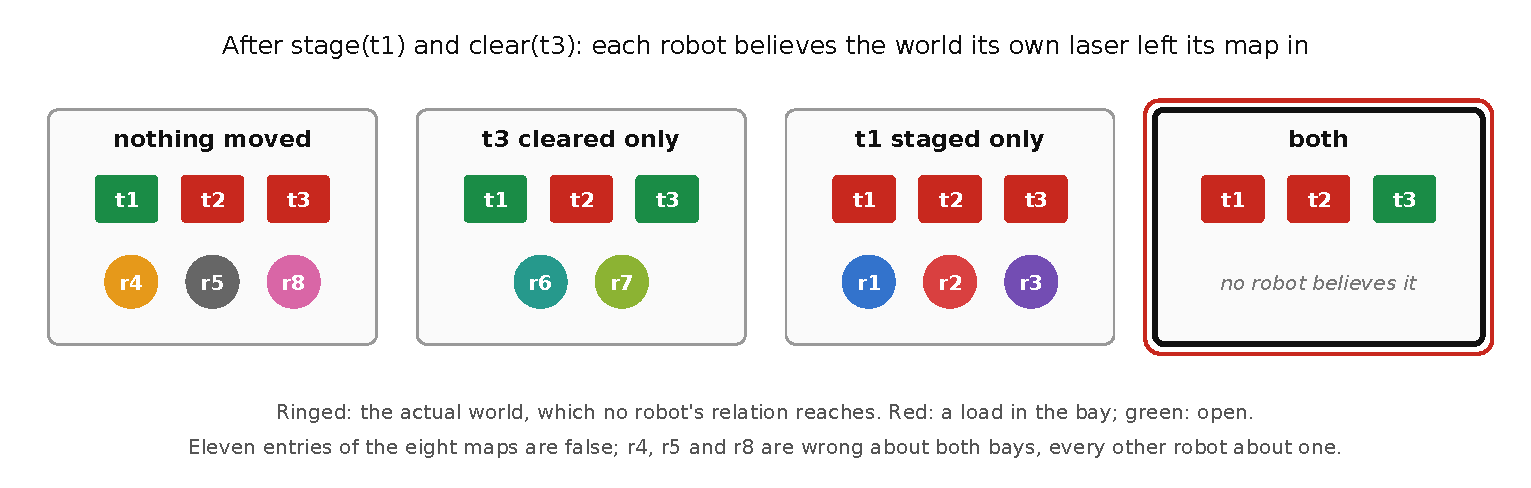
\includegraphics[width=0.92\textwidth]{figures/stale_maps_model.pdf}
\caption{The model after $\mathit{stage}(t_1)$ and $\mathit{clear}(t_3)$ on the
floor of Figure~\ref{fig:floor}. Each robot's relation leads from the actual
world, ringed, to the world its station leaves its map in.}
\label{fig:model}
\end{figure}

Each relation is a function onto a world that maps to itself, so every relation
is serial, transitive and Euclidean, and the frame is $\mathrm{KD45}_n$. On this
floor no station sees both changes, so no robot's relation reaches the actual
world. The eleven false entries of Figure~\ref{fig:model} are those of
\code{validate.sh}'s STALE check, which compares the trace's beliefs with
$\shift \oplus \Obs_i$ robot by robot.

The beliefs robots hold about each other follow:
$\Bop{i}\Bop{j}\varphi$ at $C$ is $\varphi$ at $\Obs_i \cap \Obs_j$. A robot
believes another has seen exactly the changes both of them saw. Fifteen of the 56
beliefs about another robot's map of $t_1$ are false, and twelve of $t_3$:
$r_1$ believes $r_6$'s map shows $t_3$ blocked, since $\Obs_{r_1} \cap
\Obs_{r_6} = \emptyset$, and it shows $t_3$ open.

%  ======================================================================
\section{A map sent}
\label{sec:report}

\begin{proposition}[A received map taken as a fact]
\label{prop:collapse}
Suppose $\Bop{j}\blocked(t)$ holds at the actual world and $j$ is told
$\neg\blocked(t)$ by a private announcement, $j$ Fully and every other robot
oblivious. Then after the update $j$ has no successor at the actual world, and
believes every formula.
\end{proposition}

\begin{proof}
$j$ is Fully, so from the actual world paired with the announcement's event it
reaches $(v,\mathit{pos})$ for $v \in R_j(w)$ at which $\neg\blocked(t)$ holds.
$\Bop{j}\blocked(t)$ at $w$ says there is no such $v$.
\end{proof}

\noindent
That is what fusing a received map as a fact does to a robot whose map says
otherwise. \code{validate.sh}'s COLLAPSE check shows it on $r_4$.

\begin{proposition}[The report is an update]
\label{prop:update}
Suppose $\pre(\mathit{send\text{-}open}(i,j,t))$ holds at the actual world $w$, $j$
believes $\blocked(t)$ there, and every relation is a function. Then after the
report $j$ believes $\neg\blocked(t)$, $j$'s relation is serial at every world
reachable from the actual one, $j$'s beliefs about every other bay are unchanged,
and so are every robot's beliefs other than $i$'s and $j$'s.
\end{proposition}

\begin{proof}
Let $R_j(w) = \{v\}$; $\blocked(t)$ holds at $v$, so $(v,\mathit{revise})$ exists
and is $j$'s only successor of $(w,\mathit{told})$; it differs from $v$ only in
$\blocked(t)$, now false. From $(v,\mathit{revise})$, $j$ reaches
$(u,\mathit{revise})$ for $R_j(v) = \{u\}$, and $u = v$ since $v$'s relation for
$j$ maps it to itself, so the world exists. Every other robot $k \neq i$ is
oblivious with the null event, which has trivial postconditions and occurs
everywhere, and Lemma~\ref{lem:oblivious} gives back $k$'s worlds as they were.
\end{proof}

\noindent
The sender is Fully and $\mathit{told}$ changes no atom, so its beliefs about the
bays are unchanged too; what it gains is that $j$ now believes $t$ open. The
recipient's new belief is an update in the sense of Katsuno and
Mendelzon~\cite{km1991}, not a revision in that of Alchourr\'on, G\"ardenfors and
Makinson~\cite{agm1985}: $j$'s map was right when it was made, and the world has
changed since. Plausibility models~\cite{bs2008} would revise; the logic needs
nothing beyond $\mathrm{KD45}_n$ to update.

\begin{proposition}[The guard]
\label{prop:guard}
After the forklift, if robot $i$'s map has bay $t$ wrong, then for every robot $j$,
$\Bop{i}\Bop{j}\blocked(t) \leftrightarrow \Bop{i}\blocked(t)$ holds at the actual
world. Hence neither report about $t$ from $i$ applies, to any recipient.
\end{proposition}

\begin{proof}
$i$'s map has $t$ wrong iff $t \in C \setminus \Obs_i$. By
Proposition~\ref{prop:model}, $\Bop{i}\Bop{j}\varphi$ at $C$ is $\varphi$ at
$\Obs_i \cap \Obs_j$ and $\Bop{i}\varphi$ is $\varphi$ at $\Obs_i$. Neither set
contains $t$, so $\blocked(t)$ has its shift-map value at both. The precondition
of $\mathit{send\text{-}open}$ asks $\Bop{i}\neg\blocked(t) \wedge
\Bop{i}\Bop{j}\blocked(t)$, that of $\mathit{send\text{-}blocked}$ the
reverse, and either contradicts the equivalence.
\end{proof}

\noindent
A robot that missed a change believes the forklift's slot passed with nothing
moved, and in that world every robot saw the same. So a stale reading is never
sent, and in particular never over a fresh one. GUARD checks the case:
$\mathit{send\text{-}open}(r_4, r_2, t_1)$ does not apply.

%  ======================================================================
\section{Planning}
\label{sec:planning}

The four floors were grounded by plank and solved by Aletheia with consistent
beliefs required, every policy replayed by \code{tools/trace.py}, which keeps the
submodel the designated worlds generate. The radio floor grounds to 51 atoms and
396 actions.

\begin{table}[H]
\centering\small
\begin{tabularx}{\textwidth}{@{}l X@{}}
\toprule
check & result \\
\midrule
FLOOR & the floor's three claims hold \\
STALE & after the forklift every robot believes $\shift \oplus \Obs_i$; 11 entries are false \\
RADIO & $\mathit{clear}(t_3)$, $\mathit{stage}(t_1)$, $\mathit{send\text{-}open}(r_6,r_2,t_3)$, $\mathit{cross}(r_2,t_3)$, $\mathit{send\text{-}open}(r_2,r_4,t_3)$, $\mathit{cross}(r_4,t_3)$, $\mathit{send\text{-}open}(r_2,r_8,t_3)$, $\mathit{cross}(r_8,t_3)$: 8 expansions by replanning \\
GUARD & $\mathit{send\text{-}open}(r_4, r_2, t_1)$ does not apply \\
COLLAPSE & a plain announcement to $r_4$ that $t_3$ is open leaves $r_4$ with no world \\
SILENT & no policy; the space is exhausted at depth 2 \\
DOUBT & no false belief after the forklift; the policy sends each hauler to look at $t_3$; depth 8, 3\,382 expansions \\
RESYNC & every map current, with 11 messages \\
\bottomrule
\end{tabularx}
\caption{The eight checks of \code{tools/validate.sh}, run without a simulator.}
\label{tab:checks}
\end{table}

The radio policy leaves eight entries stale, since nothing requires $r_1$, $r_3$,
$r_5$, $r_6$ and $r_7$ to hold current maps. The relay is the planner's: after
$r_6$'s report $r_2$ believes $t_3$ open and believes $r_4$ and $r_8$ hold the
shift map's reading, by Lemma~\ref{lem:oblivious}, so the precondition of its own
reports to them holds.

\begin{proposition}[The least number of messages]
\label{prop:least}
After the forklift, a policy that makes every robot believe every bay as it is
sends at least as many map reports as there are stale entries, and on the resync
floor the planner's sends exactly that many.
\end{proposition}

\begin{proof}
By Proposition~\ref{prop:update} and the remark after it, a map report changes
the recipient's belief about one bay and no robot's belief about any other.
$\mathit{cross}$ changes only $\mathit{delivered}(h)$, the forklift's actions
occur once each, and there is no other action on the floor; so each report
removes at most one stale entry, and no other action removes any. The resync
policy sends 11, the number of stale entries.
\end{proof}

%  ======================================================================
\section{Many robots}
\label{sec:scale}

\code{tools/scaling.py} draws random fleets, each robot seeing each changed bay
with probability 0.3 and a third of them hauling, and solves the radio and resync
floors, three seeds per size. Times are the planner's, measured on eight of
sixteen cores while another session's simulations ran on the rest.

\begin{table}[H]
\centering\small
\begin{tabular}{@{}r r l l l r r@{}}
\toprule
robots & haulers & stale & radio sends & resync sends & time & broadcast \\
\midrule
4 & 1 & 5--6 & 0, or no policy & 5, or no policy & 0.01\,s & 36 \\
8 & 2 & 10--13 & 2 & one per stale entry & 0.1--3\,s & 168 \\
16 & 5 & 19--24 & 2--5 & one per stale entry & 1--3\,s & 720 \\
32 & 10 & 43--52 & 7--10 & one per stale entry & 41--104\,s & 2\,976 \\
64 & 21 & 91--97 & none in 600\,s & none in 600\,s & 600\,s budget & 12\,096 \\
\bottomrule
\end{tabular}
\caption{Random fleets. Broadcast is every map of every bay to every other robot,
$N(N-1)\cdot 3$.}
\label{tab:scale}
\end{table}

Two four-robot fleets have no policy, correctly: no robot saw $t_3$ cleared, so by
Proposition~\ref{prop:model} no robot believes it open and no report about it
applies. Wherever there is a policy the resync floor's sends equal the stale
entries. The search does not scale as far as the counts. By
Proposition~\ref{prop:model} the model after the forklift has four worlds for any
fleet; what grows is the number of ground actions, $N(N-1)\cdot 3 \cdot 2$ map
reports, 24\,192 at 64 robots, over which no policy was found within the budget.

%  ======================================================================
\section{On the floor}
\label{sec:runtime}

Each robot runs a living map: the shift map, every cell observed at time zero,
into which each scan of the robot's own laser is cast from its pose. Evidence is
log-odds, updated once per cell per scan, and a cell changes class only past a
threshold; every cell carries the time it was last observed; the other robots,
whose odometry is read, are masked out of every scan. A map sent carries a
bay's cells and their observation times, and the receiver merges them by its
rule: the reading further from 50, the sender's, or the one observed later.

\begin{lemma}[Confidence cannot repair a stale map]
\label{lem:tie}
Under the rule that keeps the reading further from 50, a tie keeping the
receiver's, a received map never replaces a cell the receiver has settled as free
or occupied when its cells are written as 0 and 100.
\end{lemma}

\begin{proof}
$|0 - 50| = |100 - 50|$, so a contradicting reading is never further from 50 than
the receiver's, and the tie keeps the receiver's.
\end{proof}

\noindent
This is \code{epistemic\_slam::fuse}'s rule, with which the pass-through
demonstration exchanges maps. The observation-time rule takes each cell from
whoever saw it last; it does mechanically what Proposition~\ref{prop:update}
does, and it needs the times, which an occupancy grid does not carry. A crew node
carries out the forklift's changes, the exchanges and the hauls for every fleet,
and the epistemic fleet's performers relay their actions to it, so that the
fleets differ in what they decide and in nothing else.

%  ======================================================================
\section{Four fleets}
\label{sec:runs}

Four fleets ran on the same floor, recorded on an Xvfb display. Three share every
map of every bay with every other robot, sender by sender, merged by confidence,
by the sender's reading, or by observation time; the fourth runs the radio
policy. \code{tools/fleets.py} said what each would do before it ran, by
replaying the exchanges and driving each hauler along its route over the floor
plan with its map updated wherever the route brings a change into sight; the
mission failed any run that did otherwise, and none did.

\begin{table}[H]
\centering\small
\begin{tabular}{@{}l r r r l@{}}
\toprule
fleet & maps of a bay sent & over a fresh reading & stale after & delivered \\
\midrule
fuse & 168 & 0 & 11 & none \\
overwrite & 168 & 10 & 0 & $r_2, r_4, r_8$ \\
recency & 168 & 0 & 0 & $r_2, r_4, r_8$ \\
epistemic & 3 & 0 & 8 & $r_2, r_4, r_8$ \\
\bottomrule
\end{tabular}
\caption{The recorded runs. ``Over a fresh reading'' counts the merges that
replaced a correct reading with a wrong one; ``stale after'' the false entries
once the exchanges are done.}
\label{tab:runs}
\end{table}

In every run the forklift's changes were read on exactly the robots
Fact~\ref{fact:sight} names, within 1.8 to 4\,s. On the fuse floor $r_2$'s map
showed every bay blocked and it had no route; $r_4$ and $r_8$ set off for $t_1$,
read its load with their own lasers after 21.3 and 14.9\,m, and with $t_3$ still
blocked on their maps had no route. Overwrite delivered because the robots that
saw the changes were still looking: each of the ten stale readings written over a
fresh one was read again by the robot's own laser within seconds, before its
turn to send. With those robots no longer looking, the replay predicts that the
first sender's stale $t_3$ reaches every robot and no hauler delivers.

On the epistemic floor the view drew the model's row beside every robot's map
throughout, and at the end the mission asked the epistemic state, for every
robot and bay, whether the robot believes it blocked, open or neither. The
answers matched the robots' maps on all 24. $r_4$ and $r_8$ ended with $t_1$
still read clear: their routes through $t_3$ never brought $t_1$ into view, and
the policy never needed them to know it.

\begin{figure}[H]
\centering
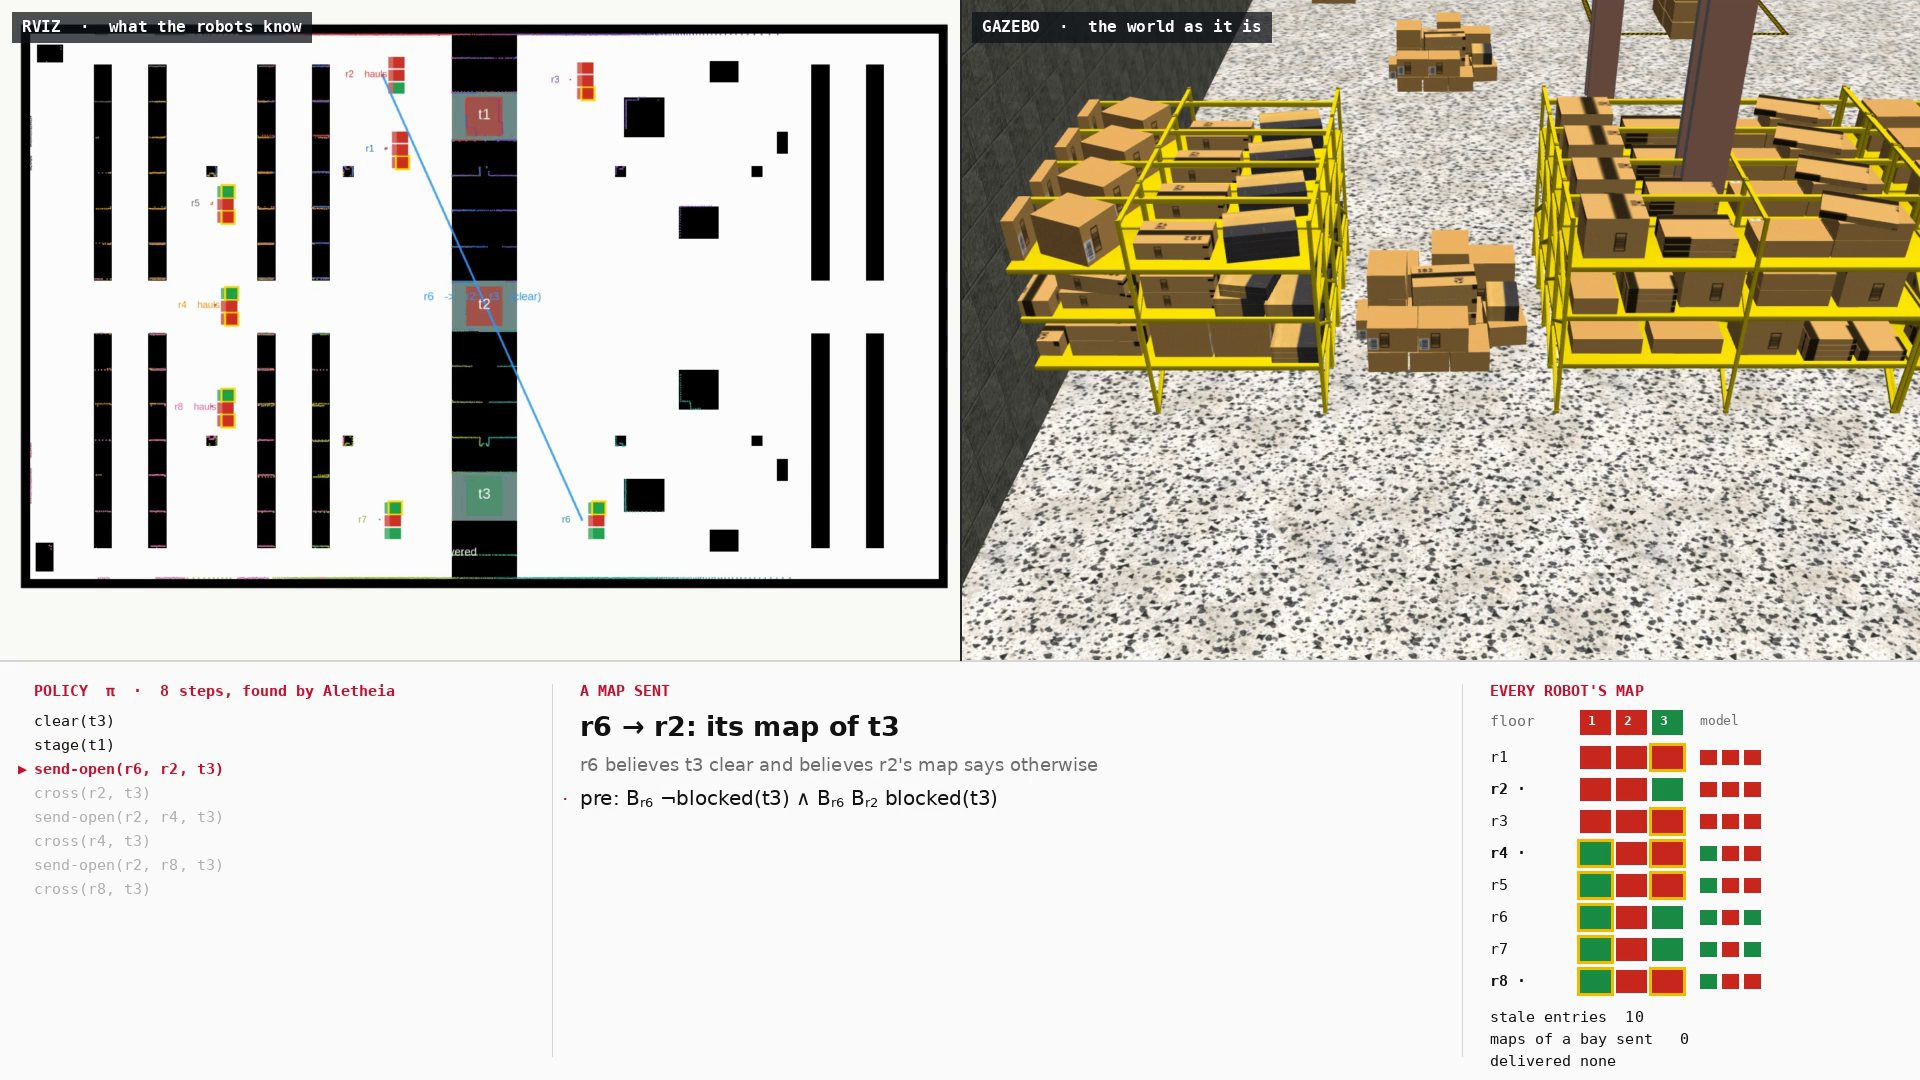
\includegraphics[width=\textwidth]{figures/stale_maps_frame.jpg}
\caption{The epistemic run as $r_6$ sends its map of $t_3$ to $r_2$. Left, RViz:
each robot's map of the three bays as three tiles, a stale tile ringed. Right,
Gazebo. Below, the policy, the step with its precondition, and every robot's map
beside the model's row.}
\label{fig:frame}
\end{figure}

%  ======================================================================
\section{Defects}
\label{sec:defects}

\paragraph{An else-if that grounds as never}
The forklift's observability was first one condition with an else-if branch for
the doubting floor. plank grounds an else-if branch without its own condition and
puts that condition and its negation into the else, so every robot that did not
see a change became doubting and none oblivious, and the radio floor came back
unsolvable at depth 2. Each change is now one action per floor.

\paragraph{A plan without its epistemic fields}
The planner plugin's best-first search returns a flat plan, and the epistemic
executor failed at its first step applying an action with no name. AO$^*$ spends
its budget over 396 ground actions before depth 8; replanning returns the eight
steps as a policy in eight expansions.

\paragraph{A map that forgot what it had just seen}
The living map first wrote a return as occupied and every crossed cell as free;
a beam grazing a load's face cleared the cell another beam had ended in, and a
hauler that had read $t_1$ blocked read it clear half a second later. Evidence is
now log-odds.

\paragraph{A prediction that froze the observers}
The first replay froze every map after the forklift and predicted that no hauler
would deliver under overwrite. The run delivered all three, for the reason given
in Section~\ref{sec:runs}, and the replay now lets an observer read its bay
before it sends.

\paragraph{Another world in the recording}
Four takes showed, in the Gazebo client, the static scene of a scenario another
session was running on the same machine, while the server simulated this floor
and the runs' data were unaffected. The two shared neither a ROS domain nor a
Gazebo master, and the cause was not established. The recorder compares the
client's opening shot with a reference and relaunches when it differs.

\paragraph{A trace that doubled}
The trace kept every world of each product update, and the resync policy's
reports took the model to 6\,208 worlds. It now keeps the generated submodel,
14 worlds for the same policy.

%  ======================================================================
\section{What this does not show}
\label{sec:limits}

\begin{itemize}[leftmargin=1.4em, itemsep=2pt]
  \item Localisation. A robot that did not know where it is would not know which
        bay it saw; that is SLAM's other half, and the model would need worlds
        for poses as well as maps.
  \item Observation the model does not contain. A hauler's map learns what its
        laser passes as it drives; the model learns only from actions. They agreed
        at the end of the recorded run, and need not in general.
  \item Communication that can fail, or a fleet beyond 32 robots planned.
\end{itemize}

\begin{thebibliography}{9}
\bibitem{agm1985} C.~E. Alchourr\'on, P.~G\"ardenfors and D.~Makinson.
On the logic of theory change: partial meet contraction and revision functions.
\emph{Journal of Symbolic Logic} 50(2):510--530, 1985.
\bibitem{bms1998} A.~Baltag, L.~S. Moss and S.~Solecki.
The logic of public announcements, common knowledge, and private suspicions.
\emph{Proceedings of TARK VII}, 43--56, 1998.
\bibitem{bs2008} A.~Baltag and S.~Smets.
A qualitative theory of dynamic interactive belief revision.
In \emph{Logic and the Foundations of Game and Decision Theory}, 11--58.
Amsterdam University Press, 2008.
\bibitem{ba2011} T.~Bolander and M.~B. Andersen.
Epistemic planning for single- and multi-agent systems.
\emph{Journal of Applied Non-Classical Logics} 21(1):9--34, 2011.
\bibitem{km1991} H.~Katsuno and A.~O. Mendelzon.
On the difference between updating a knowledge base and revising it.
\emph{Proceedings of KR}, 387--394, 1991.
\bibitem{tbf2005} S.~Thrun, W.~Burgard and D.~Fox.
\emph{Probabilistic Robotics}. MIT Press, 2005.
\bibitem{ulises2026fb} H.~Ulises.
A false belief on a warehouse floor: a relocation one robot does not see, and
the report that repairs it. Epistemic Robotics report, 2026.
\bibitem{ulises2026pt} H.~Ulises.
The pass-through problem: multi-agent epistemic planning over maps the robots
build. Epistemic Robotics report, 2026.
\end{thebibliography}

\section*{Reproduction}

\begin{lstlisting}[language={}]
ros2 launch stale_map_demo stale_maps_launch.py                 # fleet:=epistemic
ros2 launch stale_map_demo stale_maps_launch.py fleet:=fuse      # also overwrite, recency
bash tools/validate.sh                                            # eight checks
python3 tools/fleets.py                                           # what each fleet will do
python3 tools/fleets.py --transient
python3 tools/scaling.py --robots 8 16 32 64 --seeds 1 2 3
bash tools/record_demo.sh epistemic /tmp/raw.mkv /tmp/run.log
\end{lstlisting}

\end{document}
